\chapter{Implementation}\label{ch:Implementation}

This chapter examines the implementation of the project in its main stages. Firstly, the way the data was preprocessed for the model will be discussed. Then the way the model was implemented and the iterations the model went through. 

\section{Development Tools}
This section will look at the hardware and software that was used for the production of the research artefact to achieve the aims and objectives.
\subsection{Hardware}
No specialist hardware was required for this project. Only a computer was needed on the hardware side of things.
\subsection{Software}  
The software that was required for this project was a development environment to program in, the chosen development environment for this project was Jupyter Notebook. In addition to the use of a IDE, certain libraries were used for both the preprocessing of the data set and for building the actual model. The libraries needed for this project to aid in the research are listed below with an explanation of why and how they were used.
\subsubsection{Data Preprocessing Libraries}
\begin{itemize}
    \item Pandas is a library to make handling a data set easy to do by using a custom data frame type to store the data. when the data set was first received it was broken up into the races from each month for the past ten years. To leverage the data easily, the data was merged into one larger data set. Pandas was used for this and then handling the data throughout the preprocessing stage up until it was split into training and testing for the model. 
    \item Missingno was used to look at a small sample of the data set to quickly visualize the completeness of features in the data set. 
    \item pyplot is a part of the matplotlib library and was used to create graphs during the data explorations phase.
    \item seaborn was also used to create graphs, especially box plots to look at the quartile ranges of feature sets. 
    \item Label encoder  from sklearn preprocessing was used to encode the string labels to numbers so they can then be normalized for the input to the neural network.
    \item normalize was used to normalise the x values for the algorithm.
\end{itemize}
\subsubsection{Model Building Libraries}
\begin{itemize}
    \item SMOTE from imblearn oversampling was used to minimise an over fitting issue that was encountered 
    \item train test split sklearn model selection was used to split the ddata up into the training and the testing subsets.
    \item MLP classifier from sklearn neural network was the algorithm used for the neural network classification task. 
\end{itemize}
\subsubsection{Evaluation and Testing Libraries}
The below were all used to gather metrics that could be used to evaluate the model.
\begin{itemize}
    \item classification report from sklearn metrics.
    \item confusion matrix from from sklearn metrics.
    \item accuracy score from sklearn metrics.
\end{itemize}

\section{Data Preprocessing}
This section will talk through the steps taken to get the data set ready for training the leveraged algorithm to produce the research artefact.

\subsection{Loading the Dataset}
Loading the data set was done using the pandas library, the data set was loaded into a data frame to make it easy to manipulate. 

\subsection{Handling Missing Data}
The way in which missing data was handled depends on the feature, some features were deleted if that column in the data set was completely and some had values placed into the n/a that appeared in the data frame once it had been imported. Some examples of the data imputated and the reasoning for the imputated values will be mentioned now, as well as the reasoning for deleting some of the features. Some examples of the imputated data are: The feature 'actual going' had unknown as a label in the data set. Twelve thousand samples were missing due to this and unknown already being a part of the feature the value unknown was imputated for the missing values. Another value that was imutated was country was set to UK if it was unknown as all raced happened within the UK. Some of the empty values that were deleted as the were deemed to not affect the model if they had been filled in are the ones where information had to be written in or the odds of the race in a different format that had to be worked out. 

\section{Building the Model}
This section will walk through how the model was built and improved upon through several iterations. Mentioning how the models were improved and how they differ from the previous iteration. All the iterations follow the methodology previously stated that this project will follow. 

\subsection{Iteration One}
Once the data set had been preprocessed building a model could begin. The first step was too split the data into the x and y for the model, all features apart from result were the x and result was y. Result was the y variable as this was what we were trying to predict. The train test split was seventy, thirty respectively for the first iteration. The next stage was to encode all the features that were not already numbers. This was needed as you cant noramlise a non number type. the next stage of buliding the model was to noralise the input data for the neural network. this stage is important due to variables needing the same range of variance because the underlying probability density function is to be estimated with a kernel of the same width in each dimension \cite{97934}. The last stage of building the model is to fit the training data to the algorithm. The model at this stage had not been optimised and has had no parameter tuning.The results of the first iteration of this implementation are discussed below: 

Due to the feature of result having so many labels to predict in this model such as the place from first up to thirty-third in one case due to the size of that race case, as well as  labels such as being disqualified, falling, and unseating the rider as a possible race finish for a said horse, the accuracy was quite low. The accuracy as a preliminary result for the model was 0.28 or 28\%. the confusion matrix for this model can be seen below (Figure \ref{fig:M1CF}).
\begin{figure}[h!]
  \centering
  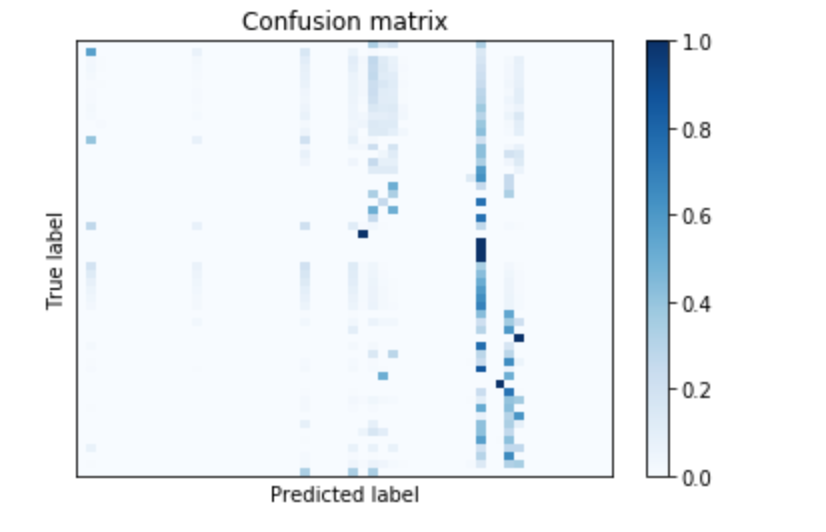
\includegraphics[width = (\textwidth)/2]{model1.png}
  \caption{Model one confusion matrix}
  \label{fig:M1CF}
\end{figure}
\subsubsection{Iteration One Conclusion}
From looking at the confusion matrix you can see the model struggles to predict the majority of the labels, which causes the model to have a low accuracy score. The improvements made in the next model is a change to the labels of the predicted feature. The results of this change is discussed below in the iteration two section. 


\subsection{Iteration Two}
As previously discussed the improvements made for the second iteration was a change to the labels it was predicting. The change that was made was the label for first place stayed the same and all other labels were changed to 0, the reasoning behind this is that for the purpose of the model any position other than first was a non winner or a loser of the race.

The way in which the label was changed was looking at any label that was not currently 1 and changing the label to 0. All other stages of building the model were the same. The data was split the same way across the same ration of training and testing. Then encoded, normalised and finally fitted to the models algorithm. The results for this iteration are as follows. The model had a greatly improved accuracy with with an accuracy score of 0.90 or 90\%. This high accuracy was caused by an over fitting of the model to the losing label. 
\begin{figure}[h!]
  \centering
  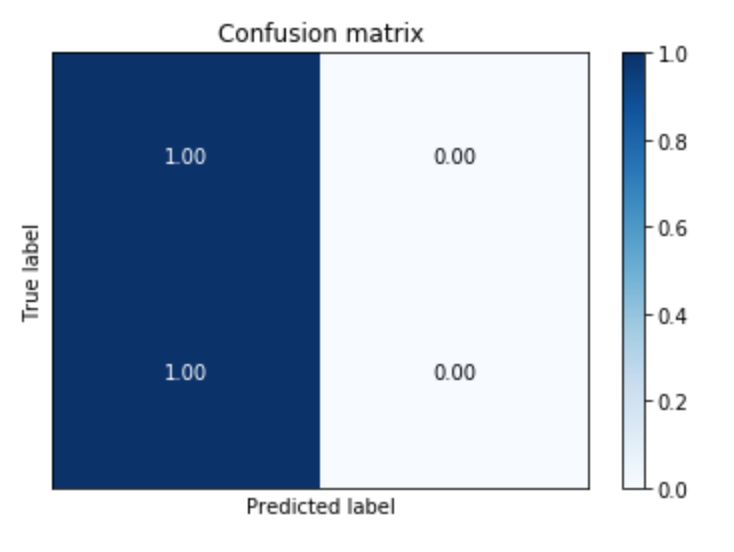
\includegraphics[width = (\textwidth)/2]{model2.png}
  \caption{Model two confusion matrix}
  \label{fig:M2CF}
\end{figure}

\subsubsection{Iteration Two Conclusion}
As you can see by the confusion matrix for this Iteration (Figure \ref{fig:M2CF}) the model was only predicting the losing label and not trying to predict the winning label at all. This is due to there being more losers to a race than a single winner so the model over fitted to that label in the predicted feature. A solution to over fitting data is implemented in the third iteration of the model. 

\subsection{Iteration Three}
The third iteration of the models implementation looks at implementing a solution to the over fitting to the loser label. The solution explored and implemented was using SMOTE. Synthetic Minority Over-sampling Technique. The way SMOTE works is by generating synthetic examples for the minority class by taking the minority class sample and introducing the synthetic one by joining any of the line segments of the k minority class neighbour \cite{SMOTE}.

This model was built slightly differently to the other two as it has SMOTE implemented. All the preprocessing of the data set is the same. The train test split is different on this model as it is moving closer to being trained on the whole data set. This time its split ninety, ten, for training and testing respectively. Then After encoding the values the same way as before, SMOTE is applied to the training data only. The reason for only over sampling the training data is so none of the testing data is used to create synthetic observations, to try and keep the results generalisable.

In using this technique to try to reduce over fitting of the loser data, some success was had. The accuracy score did drop to 0.77 or 77\%. But the precision and recall of the winner label went from 0,0 to 0.24,0.61 respectively, an improvement on before.
\begin{figure}[h!]
  \centering
  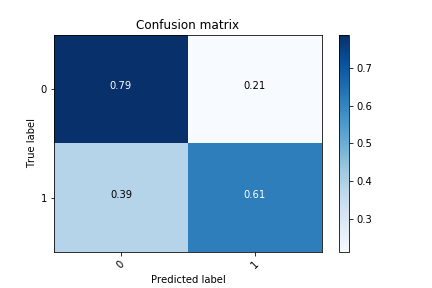
\includegraphics[width = (\textwidth)/2]{confusionMatrix.png}
  \caption{Model three confusion matrix}
  \label{fig:M3CF}
\end{figure}
\subsubsection{Iteration Three Conclusion}
As seen in the confusion matrix for the third iteration (Figure \ref{fig:M3CF}) a massive improvement on the accuracy of both predicting all labels from model one and predicting the winner from model two has been met with the implementation of changing the labels and an over-sampling technique to reduce over fitting has been achieved. But further steps need to be taken in the next iteration of the model a cross validation technique will be implemented to try and further reduce the over fitting.
\subsection{Iteration Four}
As stated previously a cross-validation technique was going to be implemented into this iteration to try and reduce the over fitting problem faced in the second iteration further. The cross validation technique used implemented in this iteration of the model is the k-fold cross validation technique. The model followed a similar implementation as the previous iterations. The data was preprocessed then a split for training data and a validation set took place on a ninety percent to ten split respectively. Then the sting labels were encoded to numbers, to then be normalised. Then SMOTE was applied to the training data to over sample the minority class of the winner label. The x values were then normalised so the neural network can accept them as the input, due to a neural network needing normalised inputs as discussed previously. The training data was then passed through the k-fold cross validation.

After the ten folds had completed the model was questioned to make a prediction. The results of the model are that it improved the accuracy score to 0.86 or 86\%, but the precision and recall of the winner label changed to 0.33, 0.42 respectively. Precision is loosely speaking how useful the results are whilst recall is how complete the results are. The confusion matrix for the model with k-fold cross validation can be seen below. 
\begin{figure}[h!]
  \centering
  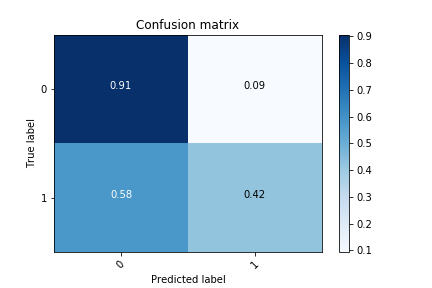
\includegraphics[width = (\textwidth)/2]{confusionMatrixkfold.png}
  \caption{Model four confusion matrix}
  \label{fig:M4CF}
\end{figure}
\subsubsection{Iteration Four Conclusions}
Implementing a cross validation technique led to an improved accuracy of the model, but the true positive score for the winning label was less than the previous iterations. This could be fixed with model optimization. the benefit of using cross validation is to reduce the chance of over fitting the model to certain classes in the data.  
\section{Conclusions}
 As seen throughout this chapter prediction models have been successfully implemented to predict the outcome of a horse race. A high level of accuracy in the later implementations has been achieved. An evaluation on the models built and the testing of the latest iteration will be discussed in the next chapter.